% Created by tikzDevice version 0.6.2-92-0ad2792 on 2013-01-11 06:07:39
% !TEX encoding = UTF-8 Unicode
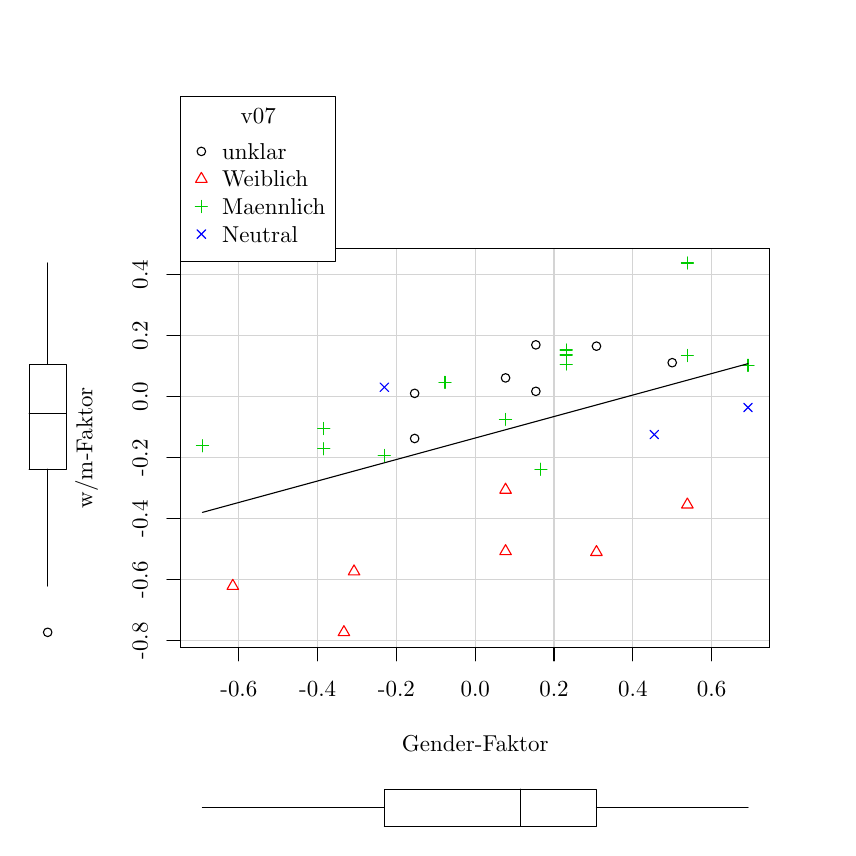
\begin{tikzpicture}[x=1pt,y=1pt]
\definecolor[named]{fillColor}{rgb}{1.00,1.00,1.00}
\path[use as bounding box,fill=fillColor,fill opacity=0.00] (0,0) rectangle (289.08,289.08);
\begin{scope}
\path[clip] (  0.00, 65.25) rectangle ( 14.45,209.40);
\definecolor[named]{drawColor}{rgb}{0.00,0.00,0.00}

\path[draw=drawColor,line width= 0.4pt,line join=round,line cap=round] (  0.54,129.51) --
	( 13.92,129.51) --
	( 13.92,167.50) --
	(  0.54,167.50) --
	(  0.54,129.51);

\path[draw=drawColor,line width= 0.4pt,line join=round,line cap=round] (  0.54,149.68) --
	( 13.92,149.68);

\path[draw=drawColor,line width= 0.4pt,line join=round,line cap=round] (  7.23, 87.32) --
	(  7.23,129.51);

\path[draw=drawColor,line width= 0.4pt,line join=round,line cap=round] (  7.23,167.50) --
	(  7.23,204.06);

\path[draw=drawColor,line width= 0.4pt,line join=round,line cap=round] (  7.23, 70.59) circle (  1.55);
\end{scope}
\begin{scope}
\path[clip] ( 55.29,  0.00) rectangle (268.16, 14.45);
\definecolor[named]{drawColor}{rgb}{0.00,0.00,0.00}

\path[draw=drawColor,line width= 0.4pt,line join=round,line cap=round] (128.88,  0.54) --
	(128.88, 13.92) --
	(205.53, 13.92) --
	(205.53,  0.54) --
	(128.88,  0.54);

\path[draw=drawColor,line width= 0.4pt,line join=round,line cap=round] (178.15,  0.54) --
	(178.15, 13.92);

\path[draw=drawColor,line width= 0.4pt,line join=round,line cap=round] ( 63.17,  7.23) --
	(128.88,  7.23);

\path[draw=drawColor,line width= 0.4pt,line join=round,line cap=round] (205.53,  7.23) --
	(260.28,  7.23);
\end{scope}
\begin{scope}
\path[clip] (  0.00,  0.00) rectangle (289.08,289.08);
\definecolor[named]{drawColor}{rgb}{0.00,0.00,0.00}

\path[draw=drawColor,line width= 0.4pt,line join=round,line cap=round] ( 76.31, 65.25) -- (247.14, 65.25);

\path[draw=drawColor,line width= 0.4pt,line join=round,line cap=round] ( 76.31, 65.25) -- ( 76.31, 60.27);

\path[draw=drawColor,line width= 0.4pt,line join=round,line cap=round] (104.79, 65.25) -- (104.79, 60.27);

\path[draw=drawColor,line width= 0.4pt,line join=round,line cap=round] (133.26, 65.25) -- (133.26, 60.27);

\path[draw=drawColor,line width= 0.4pt,line join=round,line cap=round] (161.73, 65.25) -- (161.73, 60.27);

\path[draw=drawColor,line width= 0.4pt,line join=round,line cap=round] (190.20, 65.25) -- (190.20, 60.27);

\path[draw=drawColor,line width= 0.4pt,line join=round,line cap=round] (218.67, 65.25) -- (218.67, 60.27);

\path[draw=drawColor,line width= 0.4pt,line join=round,line cap=round] (247.14, 65.25) -- (247.14, 60.27);

\node[text=drawColor,anchor=base,inner sep=0pt, outer sep=0pt, scale=  0.83] at ( 76.31, 47.32) {-0.6};

\node[text=drawColor,anchor=base,inner sep=0pt, outer sep=0pt, scale=  0.83] at (104.79, 47.32) {-0.4};

\node[text=drawColor,anchor=base,inner sep=0pt, outer sep=0pt, scale=  0.83] at (133.26, 47.32) {-0.2};

\node[text=drawColor,anchor=base,inner sep=0pt, outer sep=0pt, scale=  0.83] at (161.73, 47.32) {0.0};

\node[text=drawColor,anchor=base,inner sep=0pt, outer sep=0pt, scale=  0.83] at (190.20, 47.32) {0.2};

\node[text=drawColor,anchor=base,inner sep=0pt, outer sep=0pt, scale=  0.83] at (218.67, 47.32) {0.4};

\node[text=drawColor,anchor=base,inner sep=0pt, outer sep=0pt, scale=  0.83] at (247.14, 47.32) {0.6};

\path[draw=drawColor,line width= 0.4pt,line join=round,line cap=round] ( 55.29, 67.54) -- ( 55.29,199.88);

\path[draw=drawColor,line width= 0.4pt,line join=round,line cap=round] ( 55.29, 67.54) -- ( 50.31, 67.54);

\path[draw=drawColor,line width= 0.4pt,line join=round,line cap=round] ( 55.29, 89.60) -- ( 50.31, 89.60);

\path[draw=drawColor,line width= 0.4pt,line join=round,line cap=round] ( 55.29,111.65) -- ( 50.31,111.65);

\path[draw=drawColor,line width= 0.4pt,line join=round,line cap=round] ( 55.29,133.71) -- ( 50.31,133.71);

\path[draw=drawColor,line width= 0.4pt,line join=round,line cap=round] ( 55.29,155.77) -- ( 50.31,155.77);

\path[draw=drawColor,line width= 0.4pt,line join=round,line cap=round] ( 55.29,177.82) -- ( 50.31,177.82);

\path[draw=drawColor,line width= 0.4pt,line join=round,line cap=round] ( 55.29,199.88) -- ( 50.31,199.88);

\node[text=drawColor,rotate= 90.00,anchor=base,inner sep=0pt, outer sep=0pt, scale=  0.83] at ( 43.34, 67.54) {-0.8};

\node[text=drawColor,rotate= 90.00,anchor=base,inner sep=0pt, outer sep=0pt, scale=  0.83] at ( 43.34, 89.60) {-0.6};

\node[text=drawColor,rotate= 90.00,anchor=base,inner sep=0pt, outer sep=0pt, scale=  0.83] at ( 43.34,111.65) {-0.4};

\node[text=drawColor,rotate= 90.00,anchor=base,inner sep=0pt, outer sep=0pt, scale=  0.83] at ( 43.34,133.71) {-0.2};

\node[text=drawColor,rotate= 90.00,anchor=base,inner sep=0pt, outer sep=0pt, scale=  0.83] at ( 43.34,155.77) {0.0};

\node[text=drawColor,rotate= 90.00,anchor=base,inner sep=0pt, outer sep=0pt, scale=  0.83] at ( 43.34,177.82) {0.2};

\node[text=drawColor,rotate= 90.00,anchor=base,inner sep=0pt, outer sep=0pt, scale=  0.83] at ( 43.34,199.88) {0.4};

\path[draw=drawColor,line width= 0.4pt,line join=round,line cap=round] ( 55.29, 65.25) --
	(268.16, 65.25) --
	(268.16,209.40) --
	( 55.29,209.40) --
	( 55.29, 65.25);
\end{scope}
\begin{scope}
\path[clip] ( 14.45, 14.45) rectangle (289.08,289.08);
\definecolor[named]{drawColor}{rgb}{0.00,0.00,0.00}

\node[text=drawColor,anchor=base,inner sep=0pt, outer sep=0pt, scale=  0.83] at (161.73, 27.40) {Gender-Faktor};

\node[text=drawColor,rotate= 90.00,anchor=base,inner sep=0pt, outer sep=0pt, scale=  0.83] at ( 23.42,137.33) {w/m-Faktor};
\end{scope}
\begin{scope}
\path[clip] ( 55.29, 65.25) rectangle (268.16,209.40);
\definecolor[named]{drawColor}{rgb}{0.83,0.83,0.83}

\path[draw=drawColor,line width= 0.4pt,line join=round,line cap=round] ( 76.31, 65.25) -- ( 76.31,209.40);

\path[draw=drawColor,line width= 0.4pt,line join=round,line cap=round] (104.79, 65.25) -- (104.79,209.40);

\path[draw=drawColor,line width= 0.4pt,line join=round,line cap=round] (133.26, 65.25) -- (133.26,209.40);

\path[draw=drawColor,line width= 0.4pt,line join=round,line cap=round] (161.73, 65.25) -- (161.73,209.40);

\path[draw=drawColor,line width= 0.4pt,line join=round,line cap=round] (190.20, 65.25) -- (190.20,209.40);

\path[draw=drawColor,line width= 0.4pt,line join=round,line cap=round] (218.67, 65.25) -- (218.67,209.40);

\path[draw=drawColor,line width= 0.4pt,line join=round,line cap=round] (247.14, 65.25) -- (247.14,209.40);

\path[draw=drawColor,line width= 0.4pt,line join=round,line cap=round] ( 55.29, 67.54) -- (268.16, 67.54);

\path[draw=drawColor,line width= 0.4pt,line join=round,line cap=round] ( 55.29, 89.60) -- (268.16, 89.60);

\path[draw=drawColor,line width= 0.4pt,line join=round,line cap=round] ( 55.29,111.65) -- (268.16,111.65);

\path[draw=drawColor,line width= 0.4pt,line join=round,line cap=round] ( 55.29,133.71) -- (268.16,133.71);

\path[draw=drawColor,line width= 0.4pt,line join=round,line cap=round] ( 55.29,155.77) -- (268.16,155.77);

\path[draw=drawColor,line width= 0.4pt,line join=round,line cap=round] ( 55.29,177.82) -- (268.16,177.82);

\path[draw=drawColor,line width= 0.4pt,line join=round,line cap=round] ( 55.29,199.88) -- (268.16,199.88);
\end{scope}
\begin{scope}
\path[clip] (  0.00,  0.00) rectangle (289.08,289.08);
\definecolor[named]{drawColor}{rgb}{0.00,0.00,0.00}

\path[draw=drawColor,line width= 0.4pt,line join=round,line cap=round] ( 55.29, 65.25) --
	(268.16, 65.25) --
	(268.16,209.40) --
	( 55.29,209.40) --
	( 55.29, 65.25);
\end{scope}
\begin{scope}
\path[clip] ( 55.29, 65.25) rectangle (268.16,209.40);
\definecolor[named]{drawColor}{rgb}{0.00,0.00,0.00}

\path[draw=drawColor,line width= 0.4pt,line join=round,line cap=round] (172.68,162.52) circle (  1.55);

\path[draw=drawColor,line width= 0.4pt,line join=round,line cap=round] (139.83,140.63) circle (  1.55);

\path[draw=drawColor,line width= 0.4pt,line join=round,line cap=round] (139.83,156.93) circle (  1.55);

\path[draw=drawColor,line width= 0.4pt,line join=round,line cap=round] (183.63,157.67) circle (  1.55);

\path[draw=drawColor,line width= 0.4pt,line join=round,line cap=round] (183.63,174.46) circle (  1.55);

\path[draw=drawColor,line width= 0.4pt,line join=round,line cap=round] (205.53,173.99) circle (  1.55);

\path[draw=drawColor,line width= 0.4pt,line join=round,line cap=round] (232.90,168.02) circle (  1.55);
\definecolor[named]{drawColor}{rgb}{1.00,0.00,0.00}

\path[draw=drawColor,line width= 0.4pt,line join=round,line cap=round] (114.28, 73.00) --
	(116.36, 69.38) --
	(112.19, 69.38) --
	(114.28, 73.00);

\path[draw=drawColor,line width= 0.4pt,line join=round,line cap=round] (172.68,102.27) --
	(174.76, 98.65) --
	(170.59, 98.65) --
	(172.68,102.27);

\path[draw=drawColor,line width= 0.4pt,line join=round,line cap=round] ( 74.12, 89.73) --
	( 76.21, 86.11) --
	( 72.04, 86.11) --
	( 74.12, 89.73);

\path[draw=drawColor,line width= 0.4pt,line join=round,line cap=round] (172.68,124.48) --
	(174.76,120.86) --
	(170.59,120.86) --
	(172.68,124.48);

\path[draw=drawColor,line width= 0.4pt,line join=round,line cap=round] (117.93, 94.95) --
	(120.01, 91.33) --
	(115.84, 91.33) --
	(117.93, 94.95);

\path[draw=drawColor,line width= 0.4pt,line join=round,line cap=round] (205.53,101.95) --
	(207.62, 98.34) --
	(203.44, 98.34) --
	(205.53,101.95);

\path[draw=drawColor,line width= 0.4pt,line join=round,line cap=round] (238.38,119.13) --
	(240.47,115.52) --
	(236.29,115.52) --
	(238.38,119.13);
\definecolor[named]{drawColor}{rgb}{0.00,0.80,0.00}

\path[draw=drawColor,line width= 0.4pt,line join=round,line cap=round] (183.26,129.51) -- (187.64,129.51);

\path[draw=drawColor,line width= 0.4pt,line join=round,line cap=round] (185.45,127.32) -- (185.45,131.70);

\path[draw=drawColor,line width= 0.4pt,line join=round,line cap=round] (126.68,134.48) -- (131.07,134.48);

\path[draw=drawColor,line width= 0.4pt,line join=round,line cap=round] (128.88,132.29) -- (128.88,136.68);

\path[draw=drawColor,line width= 0.4pt,line join=round,line cap=round] (170.49,147.54) -- (174.87,147.54);

\path[draw=drawColor,line width= 0.4pt,line join=round,line cap=round] (172.68,145.34) -- (172.68,149.73);

\path[draw=drawColor,line width= 0.4pt,line join=round,line cap=round] (148.58,160.91) -- (152.97,160.91);

\path[draw=drawColor,line width= 0.4pt,line join=round,line cap=round] (150.78,158.72) -- (150.78,163.10);

\path[draw=drawColor,line width= 0.4pt,line join=round,line cap=round] (192.39,167.50) -- (196.77,167.50);

\path[draw=drawColor,line width= 0.4pt,line join=round,line cap=round] (194.58,165.31) -- (194.58,169.69);

\path[draw=drawColor,line width= 0.4pt,line join=round,line cap=round] (104.78,136.94) -- (109.17,136.94);

\path[draw=drawColor,line width= 0.4pt,line join=round,line cap=round] (106.98,134.75) -- (106.98,139.13);

\path[draw=drawColor,line width= 0.4pt,line join=round,line cap=round] (258.09,167.06) -- (262.47,167.06);

\path[draw=drawColor,line width= 0.4pt,line join=round,line cap=round] (260.28,164.87) -- (260.28,169.26);

\path[draw=drawColor,line width= 0.4pt,line join=round,line cap=round] (104.78,144.27) -- (109.17,144.27);

\path[draw=drawColor,line width= 0.4pt,line join=round,line cap=round] (106.98,142.07) -- (106.98,146.46);

\path[draw=drawColor,line width= 0.4pt,line join=round,line cap=round] (236.19,204.06) -- (240.57,204.06);

\path[draw=drawColor,line width= 0.4pt,line join=round,line cap=round] (238.38,201.87) -- (238.38,206.25);

\path[draw=drawColor,line width= 0.4pt,line join=round,line cap=round] ( 60.98,138.03) -- ( 65.37,138.03);

\path[draw=drawColor,line width= 0.4pt,line join=round,line cap=round] ( 63.17,135.84) -- ( 63.17,140.22);

\path[draw=drawColor,line width= 0.4pt,line join=round,line cap=round] (192.39,170.81) -- (196.77,170.81);

\path[draw=drawColor,line width= 0.4pt,line join=round,line cap=round] (194.58,168.61) -- (194.58,173.00);

\path[draw=drawColor,line width= 0.4pt,line join=round,line cap=round] (236.19,170.64) -- (240.57,170.64);

\path[draw=drawColor,line width= 0.4pt,line join=round,line cap=round] (238.38,168.45) -- (238.38,172.83);

\path[draw=drawColor,line width= 0.4pt,line join=round,line cap=round] (192.39,172.61) -- (196.77,172.61);

\path[draw=drawColor,line width= 0.4pt,line join=round,line cap=round] (194.58,170.42) -- (194.58,174.80);
\definecolor[named]{drawColor}{rgb}{0.00,0.00,1.00}

\path[draw=drawColor,line width= 0.4pt,line join=round,line cap=round] (258.73,150.28) -- (261.83,153.38);

\path[draw=drawColor,line width= 0.4pt,line join=round,line cap=round] (258.73,153.38) -- (261.83,150.28);

\path[draw=drawColor,line width= 0.4pt,line join=round,line cap=round] (224.88,140.50) -- (227.98,143.60);

\path[draw=drawColor,line width= 0.4pt,line join=round,line cap=round] (224.88,143.60) -- (227.98,140.50);

\path[draw=drawColor,line width= 0.4pt,line join=round,line cap=round] (127.33,157.61) -- (130.43,160.71);

\path[draw=drawColor,line width= 0.4pt,line join=round,line cap=round] (127.33,160.71) -- (130.43,157.61);
\definecolor[named]{drawColor}{rgb}{0.00,0.00,0.00}

\path[draw=drawColor,line width= 0.4pt,line join=round,line cap=round] ( 63.17,113.93) --
	(260.28,167.67);
\end{scope}
\begin{scope}
\path[clip] ( 14.45, 14.45) rectangle (289.08,289.08);
\definecolor[named]{drawColor}{rgb}{0.00,0.00,0.00}
\definecolor[named]{fillColor}{rgb}{1.00,1.00,1.00}

\path[draw=drawColor,line width= 0.4pt,line join=round,line cap=round,fill=fillColor] ( 55.29,264.28) rectangle (111.31,204.52);

\path[draw=drawColor,line width= 0.4pt,line join=round,line cap=round] ( 62.76,244.36) circle (  1.55);
\definecolor[named]{drawColor}{rgb}{1.00,0.00,0.00}

\path[draw=drawColor,line width= 0.4pt,line join=round,line cap=round] ( 62.76,236.81) --
	( 64.85,233.19) --
	( 60.67,233.19) --
	( 62.76,236.81);
\definecolor[named]{drawColor}{rgb}{0.00,0.80,0.00}

\path[draw=drawColor,line width= 0.4pt,line join=round,line cap=round] ( 60.57,224.44) -- ( 64.95,224.44);

\path[draw=drawColor,line width= 0.4pt,line join=round,line cap=round] ( 62.76,222.25) -- ( 62.76,226.63);
\definecolor[named]{drawColor}{rgb}{0.00,0.00,1.00}

\path[draw=drawColor,line width= 0.4pt,line join=round,line cap=round] ( 61.21,212.93) -- ( 64.31,216.03);

\path[draw=drawColor,line width= 0.4pt,line join=round,line cap=round] ( 61.21,216.03) -- ( 64.31,212.93);
\definecolor[named]{drawColor}{rgb}{0.00,0.00,0.00}

\node[text=drawColor,anchor=base,inner sep=0pt, outer sep=0pt, scale=  0.83] at ( 83.30,254.32) {v07};

\node[text=drawColor,anchor=base west,inner sep=0pt, outer sep=0pt, scale=  0.83] at ( 70.23,241.50) {unklar};

\node[text=drawColor,anchor=base west,inner sep=0pt, outer sep=0pt, scale=  0.83] at ( 70.23,231.54) {Weiblich};

\node[text=drawColor,anchor=base west,inner sep=0pt, outer sep=0pt, scale=  0.83] at ( 70.23,221.58) {Maennlich};

\node[text=drawColor,anchor=base west,inner sep=0pt, outer sep=0pt, scale=  0.83] at ( 70.23,211.62) {Neutral};
\end{scope}
\end{tikzpicture}
